\subsection{Seismokardiografi}
Ikke alle diagnostiseringsmetoder er brugbare som telemedicin da undersøgelsen foregår i eget hjem. Det er derfor vigtigt at gøre brug af et brugervenligt diagnostiseringsmetode der nemt kan benyttes uden opsyn af sundhedsfagligtpersonale. Seismokardiografi (SCG) falder inde for sådan kriterier.
SCG er en non-invasiv metode udviklet til at optage og analysere hjertets aktivitet som et mål for hjertets sammentrækningsevne. Hjertemuskulaturen og blodets bevægelse producerer vibrationer der transmitteres til brystvæggen som kan måles med et SCG-system. SCG repræsenterer dermed de lokale vibrationer af brystkassen som respons til hjerteslaget \cite{inan2015}.

Oprindeligt blev SCG foreslået som et diagnostisk værktøj i klinikken, hvor en læge på baggrund af målinger kunne foretage en diagnose vedrørende patientens kardiovaskulære tilstand \cite{starr1939}. Den større variabilitet i signalerne mellem patienterne har dog hæmmet denne tilgang, især i betragtning af de begrænsede værktøjer der var til rådighed på det tidspunkt. Værktøjerne er sidenhen blevet effektiviseret, og senere undersøgelser har vist at variabilitet over en serie af målinger er lav mellem personens egne målinger \cite{inan2009}, undtagen ved tilstedeværelsen af ændringer i den kardiovaskulære tilstand \cite{inan2015}. Af denne grund er SCG blev foreslået som redskab til at overvåge ændringer hos den samme patient over tid. På den måde vil patienten virke som egen kontrol, hvor variationen ikke længere er en hindring. Det har vist sig at amplituden i SCG-signaler modulerer med ændringer i den venstre ventrikulære funktion, især ændringer i slagvolumen eller minutvolumen \cite{inan2015}.\\
SCG som et bærbart målingsystem har den primære fordel at det gøres muligt at opsamle data løbende i dagligdagen, som potentielt kan hentes i ethvert miljø. Dette gør det muligt at vurdere en persons kardiovaskulære præstation under forskellige miljømæssige forhold \cite{inan2015}. Moderne SCG-systemer er i stand til at monitorere langsomme, longitudinale hjertefunktioner forbundet med et antal hjerte-karsygdomme. Detektion af subtile ændringer i hjerte patofysiologien kan potentielt gøre det muligt at justere lægemiddeldosering, hvilket kan reducere dyre og morbide genindlæggelser. \cite{munir2008}

%Signifikant features ved SCG bølgerne blev identificeret og associeret med nøglebegivenheder i hjerte cyklusen [17].
%Definering af bestemte tidsintervaler forbundet med hjertecyklusen kombineret med evnen til at foretage præcis gentagende målinger med SCG gjorde det muligt at udføre klinisk relevant tværsnits undersøgelser. Efterfølgende blev kliniske undersøgelser gennemført til at afgøre, om SCG kunne bruges til at identificere ændringer i SCG bølgen som følge af myokardisk iskæmi [99]. SCG's kliniske anvendelig  blev først vist i kilde [100]. En stor multicenter undersøgelse viste, at når man kombinerede ECG og SCG, så vil den forudsigende nøjagtighed ved at detektere fysiologiske signifikant koronararteriesygdomme øget signifikant ift. til ECG alene [7].
%Der har været meget forskning omkring SCG gennem 1900'erne, men pga. fremkomsten af ekkokardiografi og MRI, og alt for stor hardware så blev SCG stort set opgivet af det medicinske samfund [8]. Idag har den teknologiske udvikling gjort det nemmere/simplify måling og vurdering af disse signaler samt åbnet nye perspektiver \cite{inan2015}

SCG kan detekteres ved at placere et accelerometer på brystkassen og måles i enheden milli-g (mg). Ved anvendelsen af et tre-aksialt accelerometer, vil SCG komponenterne være til stede i alle tre akser, som hver viser et specifikt mønster. \cite{migeotte2012} Størstedelen af studierne omhandlende SCG fokuserer dog kun på amplituden af dorso-ventral komponenten. Da SCG tager udgangspunkt i lokale vibrationer, er det vigtigt at systemet placeres præcist, hvoraf den mest udbredte placering er sternum. \cite{pandia2012}

Signalet indeholder en ultra-lavfrekvent komponent korresponderende til bevægelsen af brystvæggen og en højfrekvent SCG komponent korresponderende til vibrationer af brystkassen pga. hjerteslaget. Et studie foretaget af Zanetti og Salerno \cite{zanetti1991} over en række måneder viste at SCG-signaler målt på sternum er stabile og er i stand til at detektere akut og kroniske ændringer i venstre ventrikulær funktion. Castigloni et al. \cite{castiglioni2007} demonstrerede at SCG-signaler fra sternum kan brydes ned i lavfrekvente (<20 Hz) komponenter relateret til minutvolumen og højfrekvente (>20 Hz) komponenter relateret til hjertelyde. 

SCG-målinger kan påvirkes af adskillige støjkilder og interferens, såsom sensor og kredsløbs støj, og bevægelsesartefakter \cite{pandia2010}. SCG repræsenterer signaler som indeholder lavfrekvente informationer, hvilket kan medføre støj. Derudover har mange syge og ældre personer en lavere signal amplitude sammenlignet med den yngre befolkning. \cite{starr1961} 

%Bevægelsesartefakter hos personer som står op under måling repræsenterer den potentielt største forhindring til at opnå pålidelig målinger. I modsætning til seng eller stol systemer, hvor personen generelt forbliver stille under målingen. Postural sving kan skabe uønskede peaks og forvrængning i de målte signaler [76,80].  Pandia et al. præsenterer foreløbige metoder til at annullere bevægelsesartefakter i SCG signaler hos gående personer, hvilket har forbedret den overordnede detektion af hjerteslaget \cite{pandia2010}. Derudover blev det observeret at lavfrekvent støj i SCG bølger kunne opnås hos en person som sad i en metro, mens et tog kørte forbi [21]. 

Et SCG kan sammenholdes med eksempelvis elektrokardiografi (EKG), phonokardiografi (PCG) og ballistokardiografi (BCG). EKG’et er det mest brugte, og viser den elektriske aktivering af hjertet. Dette kommer til udtryk i en graf, hvor fem primære begivenheder beskrives. Disse begivenheder, samlet kaldet PQRST, opstilles over SCG’et, ud fra viden om hvad de forskellige bølger i SCG’et repræsenterer. Et EKG sammenholdt med SCG, hvorpå de mekaniske begivenheder er angivet, se figur \ref{ecgscg}. \\

\begin{figure}[H]
\centering
  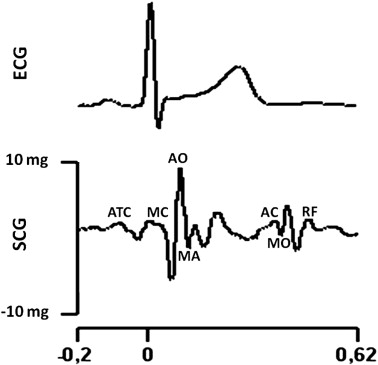
\includegraphics[width=0.6\textwidth]{Billeder/dirienzoetal2013.png}
   \caption{Et EKG sat over SCG. Taget fra Di Rienzo et al., 2013 \cite{di2013wearable}.} 
   \label{ecgscg}
\end{figure}

Følgende annotationer, som beskriver den mekaniske aktivitet i hjertet, er fremsat af Crow et al., 1994 \cite{crow1994relationship}\cite{paukkunen2014seismocardiography}:
\begin{itemize}
    \item AS, peak of atrial systole, her betegnet ATC for atrial contraction
    \item MC, mitral valve closure
    \item IM, isovolumic movement, her ikke-angivne dal mellem MC og AO, foreslået IVC for isovolumic contraction af Akhbardeh et al., 2009 \cite{akhbardeh2009comparative}
    \item AO, aortic valve opening
    \item IC, isotonic contraction, her angivet MA for den maximal acceleration, foreslået af Gurev et al., 2012 \cite{gurev2012mechanisms}
    \item RE, peak of rapid systolic ejection, her ikke-angivne bølge efter MA
    \item AC, aortic valve closure
    \item MO, mitral valve opening
    \item RF, peak of rapid diastolic filling
\end{itemize}

Disse annotationer bruges videre ud fra kendskab om hjertets virkemåde, herunder hjertets cyklus.
Hjertets cyklus opdeles i to perioder, den systoliske og diastoliske periode. Den systoliske periode indeholder PEP, IVCT og LVET. Den diastoliske periode indeholder IVRT. \cite{di2013wearable}

\textbf{PEP, pre-ejection period}, er defineret som tiden mellem Q-bølgen i EKG’et, og åbningen af aortaklappen. Denne indeholder bl.a. IVCT, og er tiden fra kontraktion af ventriklen sker, og frem til at udpumpning af blod kan forløbe grundet aortaklappens åbningen. Større PEP kan være en indikator for venstresidet hjertesvigt, som følge af lavere evne til sammentrækning. \cite{di2013wearable}

\textbf{IVCT, den isovolumetriske kontraktionstid}, er defineret som tiden mellem lukningen af mitralklappen, og åbningen af aortaklappen. Som navnet angiver, sker der ikke nogen volumetrisk ændring i denne periode. Der sker hverken en til- eller frastrømning fra venstre ventrikel. Da der sker en kontraktion, øges trykket imidlertid, hvilket hjælper med at føre blodet ud i aorta i den efterfølgende LVET periode. \cite{di2013wearable}

\textbf{LVET, left ventricular ejection time}, er defineret som tiden mellem åbningen og lukningen af aortaklappen. Denne periode beskriver derved udstrømningen af blod til aorta fra ventriklen. Som ved PEP, er denne også en indikator for venstresidet hjertesvigt, hvor lavere evne til sammentrækning fremkommer som en forlængelse af denne periode. \cite{di2013wearable}

\textbf{IVRT, den isovolumetriske reflektionstid}, er defineret som tiden mellem lukningen af aortaklappen og åbningen af mitralklappen. Som navnet angiver, sker der ikke nogen volumetrisk ændring i denne periode. Der sker hverken en til- eller frastrømning fra venstre ventrikel. Da der sker en afslapning af ventriklen, skabes et undertryk, hvilket hjælper med at føre blod ind i ventriklen ved den efterfølgende åbning af mitralklappen. \cite{di2013wearable}
 
De beskrevne perioder kan illustreres ved brug af et udvidet Wiggers diagram, hvor SCG’et er inkluderet, se figur \ref{wigdiagram}.

\begin{figure}[H]
\centering
  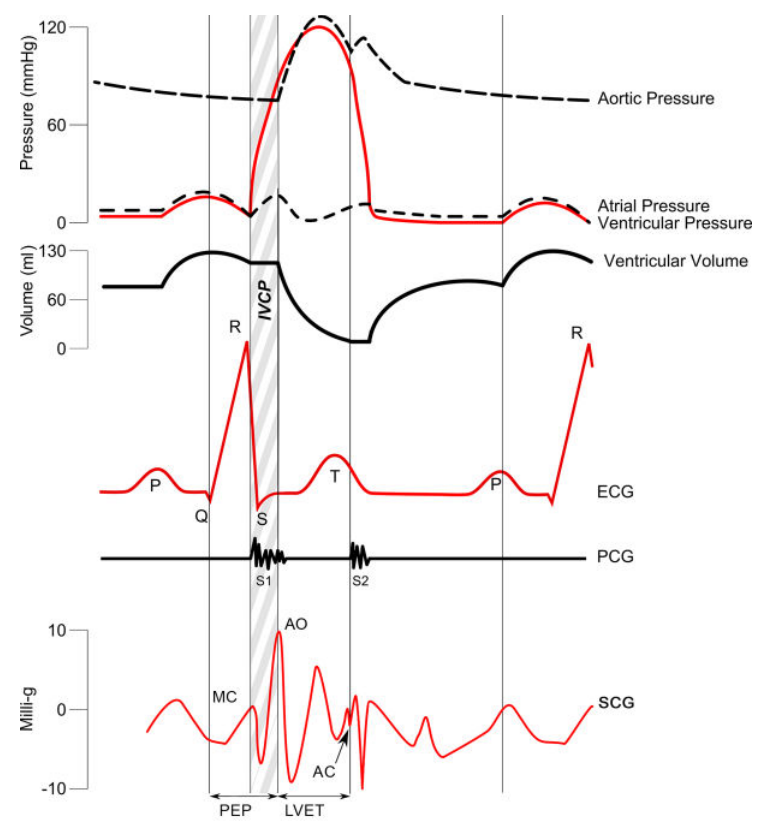
\includegraphics[width=0.7\textwidth]{Billeder/WiggersmedSCGZanetti.PNG}
   \caption{Et modificeret Wigger's diagram, hvor SCG er tilføjet. Tryk i ventrikel, atrie og aorta, samt volumen i ventriklen er vist. Yderligere er enkelte vigtige annotationer for SCG’et angivet. Taget fra Zanetti og Tavakolian, 2013 \cite{zanetti2013seismocardiography}.} 
   \label{wigdiagram}
\end{figure}

På figur \ref{wigdiagram} kan ses ændringerne i tryk og volumen, som følge af de mekaniske aktiviteter. Der ses en forøgelse i ventrikulært tryk, som følge af isovolumetrisk kontraktion, en forøgelse i aortisk tryk samt fald i ventrikulært volumen følgende isovolumetrisk kontraktion, samt stort fald i ventrikulært tryk som følge af isovolumetrisk relaksation. Isovolumetrisk relaksation er ikke illustreret, men dækkende fra starten til slutningen af anden hjertelyd på PCG’et, S2, og markerer slutningen af systolen og starten på diastolen \cite{zanetti2013seismocardiography}.


%[DER SKAL SÆTTES KILDER PÅ, OG SÅ SKAL AFSNITTET OVERORDNET REVURDERES IFT. GENTAGELSER, RENERE SPROG, DEFINITIONER (DANSK/ENGELSK NAVN) ETC.]\\
%Primære kilde ift. billede og beskrivelse: https://www-sciencedirect-com.zorac.aub.aau.dk/science/article/pii/S1566070213000805


\section{QRS kompleks signaler sammenlignet med SCG }




\begin{itemize}
\item Shafiq: Automatisk peak detektion ved brug af algoritmer 
\item Rienzo: I et studie foretaget af Rienzo et al, blev PEP og LVET undersøgt for deres stabilitet i forskellige fysiske aktiviteter. Ved brug af en kombination af EKG og SCG (Magic-SCG) blev disse STI parametre målt som er kendte for hjertets kontraktilitet. De fandt, at denne metode/ dette udstyr til at måle disse parametre var gode og robuste overfor støj.
\item Etemadi: Denne gruppe har undersøgt BCG til at måle vibrationer fra kroppen, hvorfra hjerte-mekaniske parametre kan udledes (CO, BP, contractility). Samtidig er BCG et billigt alternativ i hele befolkningen.
Gruppen har sammenlignet to typer af systemer; Elektroder på sternum: Måler STI (PEP, ændringer i CO) Ur: Måler pulse transmit time (PTT)  altså den tid det tager fra AO til det bliver opfanget af uret. Herfra beregnes BP
Desuden kommer de ind på alogritmer til at minimere bevægelsesartifaktor osv.
BCG blev målt sammen med EKG
SCG blev målt og bruger også PPG (prototype)
\item Sahoo: Fokusere på CHD og ikke HF, ECG + SCG sensorer bruges. Optager ikke med en smartphone men kan sende og kommunikere med en smart device. Sendes med bluetooth
\end{itemize}